\documentclass[9pt]{article}

\usepackage{amssymb}
\usepackage{amsmath}
\usepackage{amsfonts}
\usepackage{comment}
\usepackage{fancyhdr}
\usepackage{mathrsfs}
\usepackage{enumitem}
\usepackage{graphicx}

\usepackage{tikz}

\voffset = -50pt
%\textheight = 700pt
\addtolength{\textwidth}{60pt}
\addtolength{\evensidemargin}{-30pt}
\addtolength{\oddsidemargin}{-30pt}
%\setlength{\headheight}{44pt}

\newcommand{\qed}{\hfill \ensuremath{\Box}}


\newcommand*\circled[1]{\tikz[baseline=(char.base)]{
            \node[shape=circle,draw,inner sep=2pt] (char) {#1};}}

\newcommand{\Z}{\mathbb{Z}}
\newcommand{\I}{\mathbb{I}}
\newcommand{\M}{\mathbb{M}}
\newcommand{\R}{\mathbb{R}}
\newcommand{\C}{\mathbb{C}}
%\setcounter{section}{-1}

\begin{document}
\topskip0pt
\vspace*{\fill}
\begin{center}
{\Huge \begin{tabular}{@{}ll@{}}
   Class: & CECS 201, Section 7 \\ \\ \\
   Lab: & 3 \\ \\ \\
   Title: & Logic Gates \\ \\ \\
   Student Name: & Barry Joseph Okonoboh \\ \\ \\
   Due Date: & 16, March 2015 \\ \\ \\
   Instructor: & Dan Cregg
\end{tabular}}
\end{center}
\vspace*{\fill}
\newpage
\begin{enumerate}
%%%%%%%%%%%%%%%%%%%%%%%%%%%%%%%%%%%%%%%%01%%%%%%%%%%%%%%%%%%%%%%%%%%%%%%%%%%%%%%
   \item[b.] \textbf{Introduction.} This lab involves observing the outputs of
             the AND, OR, NAND, NOR, NOT and XOR logic gates, with varying
             input.
   \item[c.] \textbf{Project Description.} This lab has a single schematic that
            includes the six gates mentioned above. There are two inputs, A and
            B, and they are both connected to the inputs of all the gates. Each
            output of the gates in the schematic is mapped to exactly one LED,
            so that its behavior may be observed upon altering the inputs.
  	\item[d.] \textbf{Schematic.}
             \begin{center}
                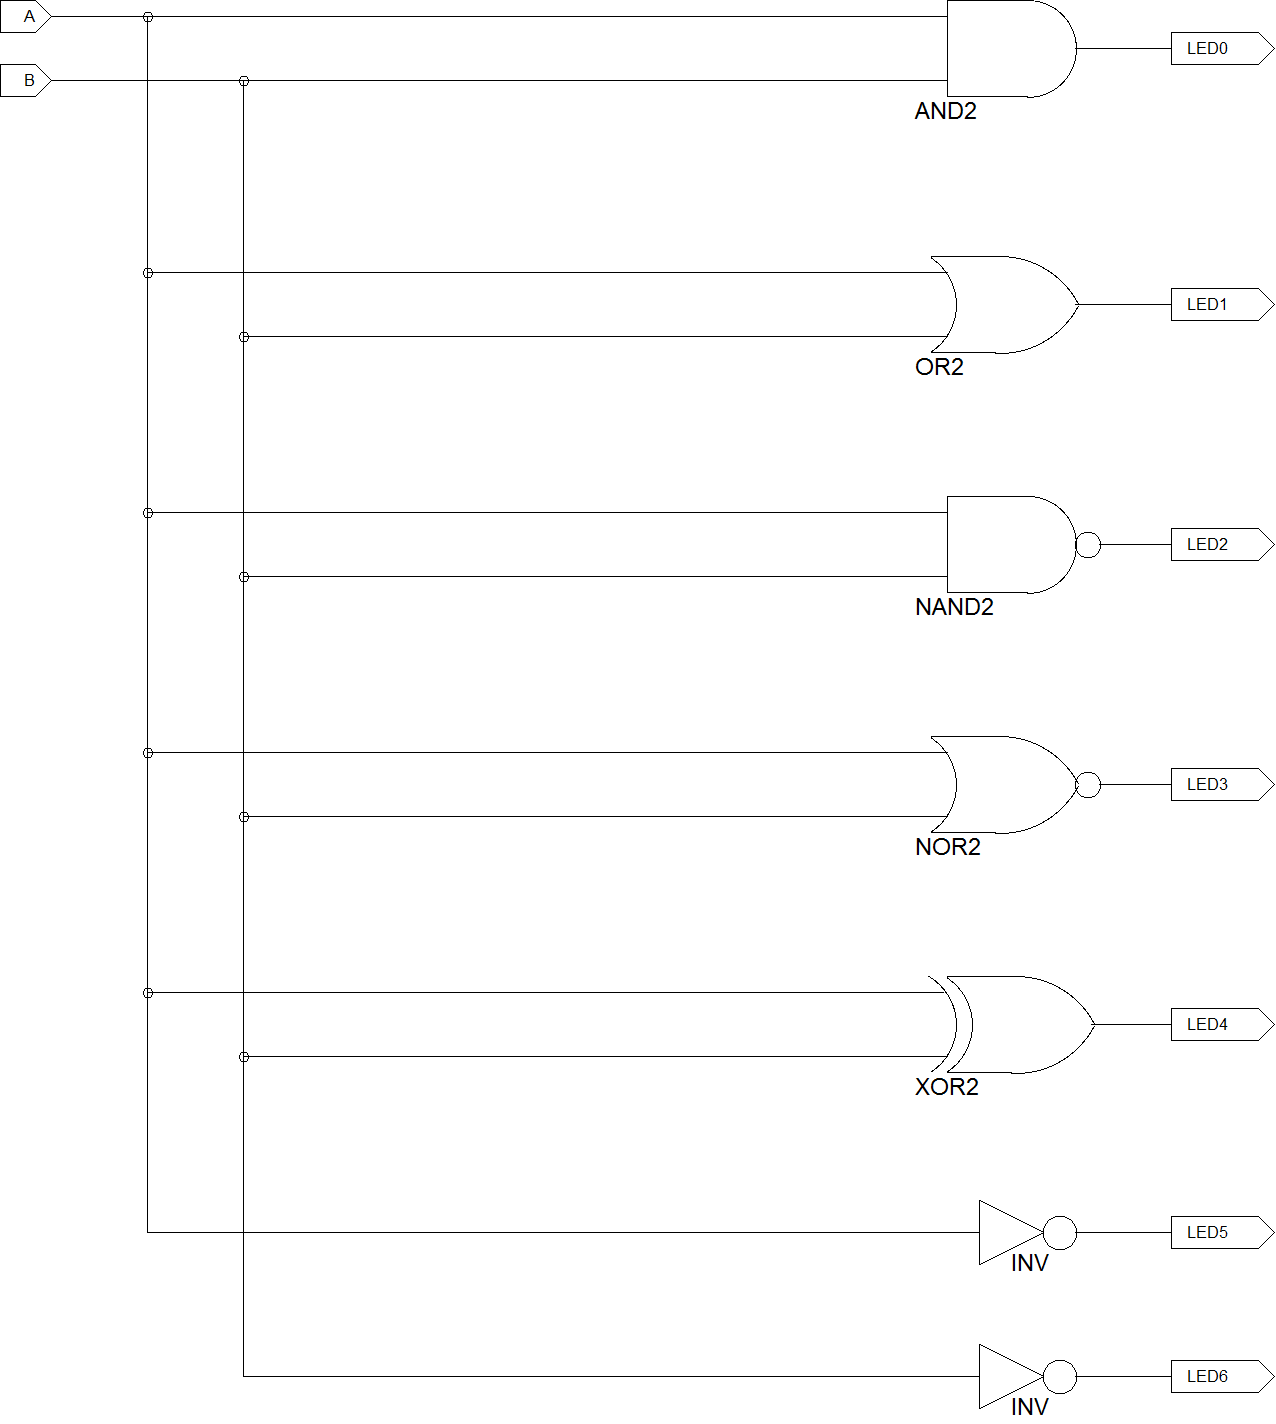
\includegraphics[width=\textwidth]{schematic.png}
             \end{center}
             
             \textbf{Truth Table.}   
   
   \begin{center}
    \begin{tabular}{@{}|c|c|c|c|c|c|c|c|@{}}
   \hline
   $A$ & $B$ & $AB$ & $A+B$ & $\overline{AB}$ & $\overline{A+B}$ & $A \oplus B$ & $\overline{A}$ \\ 
   \hline
   0 & 0 & 0 & 0 & 1 & 1 & 0 & 1 \\
   \hline
   0 & 1 & 0 & 1 & 1 & 0 & 1 & 1 \\
   \hline
   1 & 0 & 0 & 1 & 1 & 0 & 1 & 0 \\
   \hline
   1 & 1 & 1 & 1 & 0 & 0 & 0 & 0 \\
   \hline
\end{tabular}
   \end{center}
\end{enumerate}
\end{document}